
\documentclass[11pt,letterpaper]{article}

% Load some basic packages that are useful to have
% and that should be part of any LaTeX installation.
%
% be able to include figures
\usepackage{graphicx}
% get nice colors
\usepackage{xcolor}

% change default font to Palatino (looks nicer!)
\usepackage[latin1]{inputenc}
\usepackage{mathpazo}
\usepackage[T1]{fontenc}
% load some useful math symbols/fonts
\usepackage{latexsym,amsfonts,amsmath,amssymb}

% comfort package to easily set margins
\usepackage[top=1in, bottom=1in, left=1in, right=1in]{geometry}

% control some spacings
%
% spacing after a paragraph
\setlength{\parskip}{.15cm}
% indentation at the top of a new paragraph
\setlength{\parindent}{0.0cm}


\begin{document}

\begin{center}
\Large
Ay190 -- Worksheet 7\\
Anthony Alvarez\\
Date: \today
\end{center}

\section{Monte Carlo Methods}
\subsection{Measuring $\pi$ with MC Experiment}

First we implement an MC experiment to calculate the value of $\pi$. Scatter 
points randomly on the square defined by $(-0.5,-0.5)$ and $(0.5,0.5)$ and if 
$x^2 + y^2 < \frac{1}{4}$ then the point is inside the circle. We can use the 
fraction of points inside as the area and from that determine the value of 
$\pi$. 

First we use numpy's random module with a seed of 1. We can see 
~\ref{fig:nprand} that the method does seem to converge but not very quickly 
and has a great amount of noise. When we sqitch to use the SystemRandom
a function which uses the operating system to provide random numbers. This may
be more random and therefore better. However, we can see that in ~\ref{fig:sys}
that this method does have a lot of noise and doesn't seem to converge as well
as numpy's random did. 

\begin{figure}[bth]
\centering
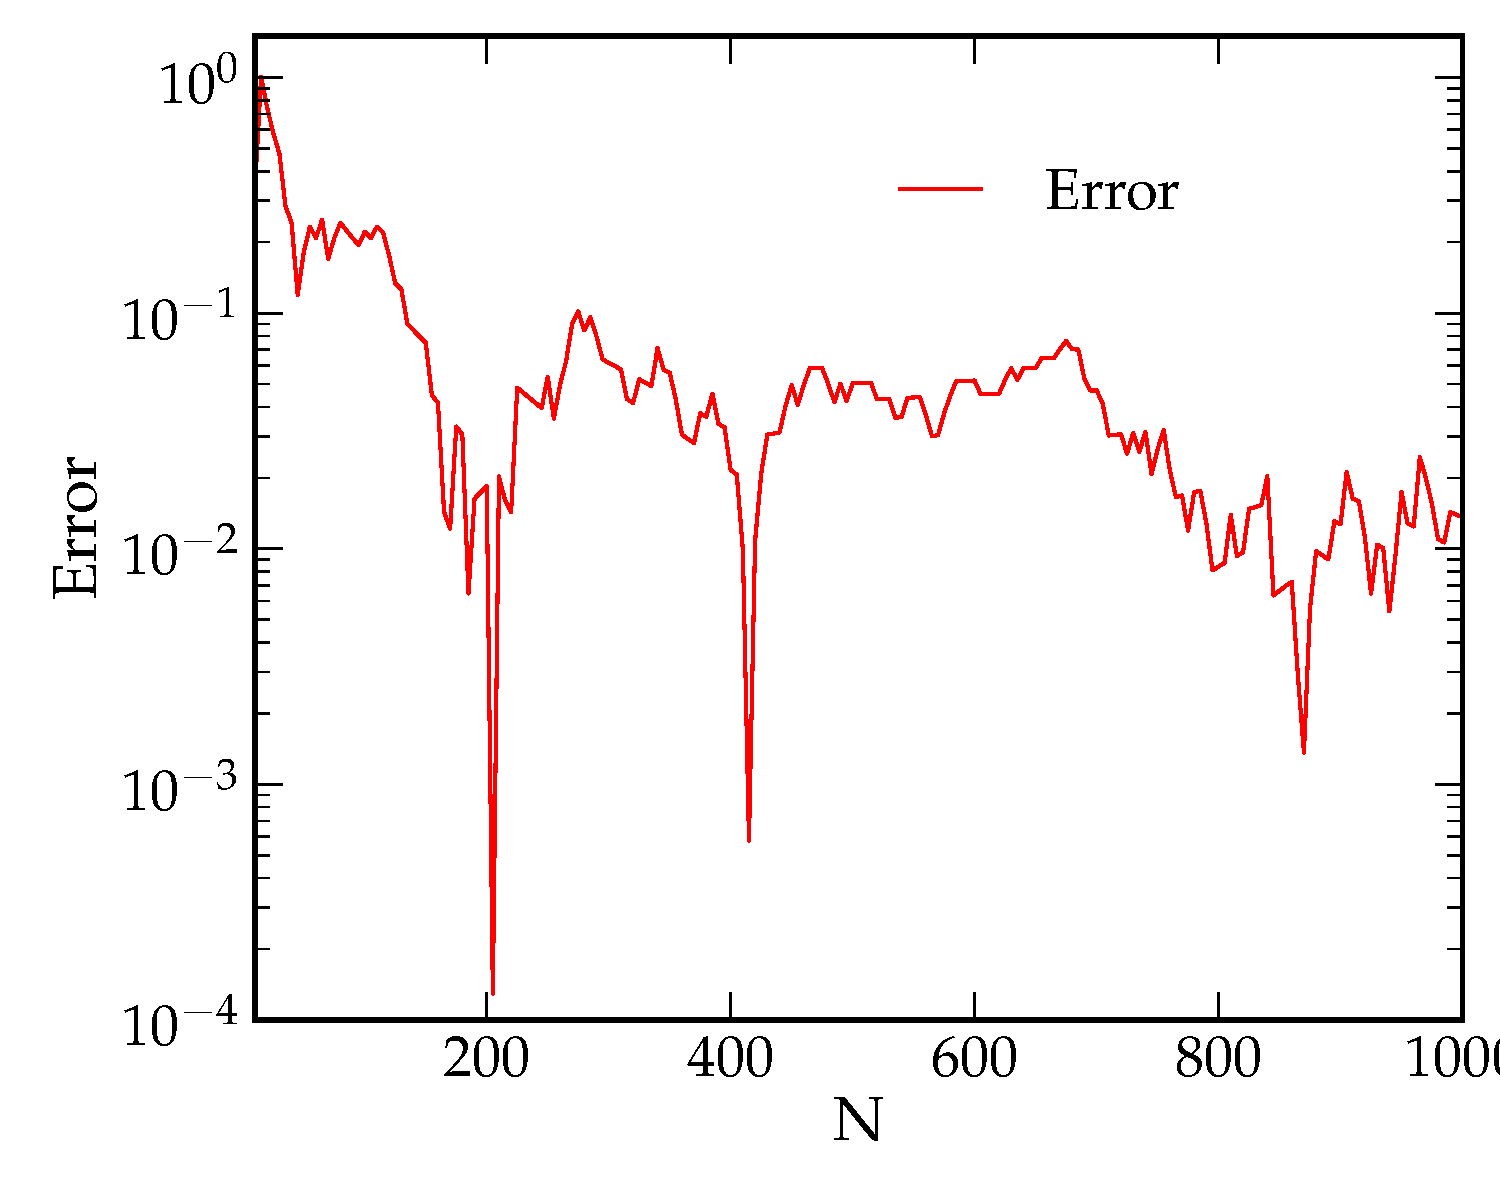
\includegraphics[width=0.5\textwidth]{1a.pdf}
\caption{Convergance of Pi by MC experimental methods using numpy random.}
\label{fig:nprand}
\end{figure}

\begin{figure}[bth]
\centering
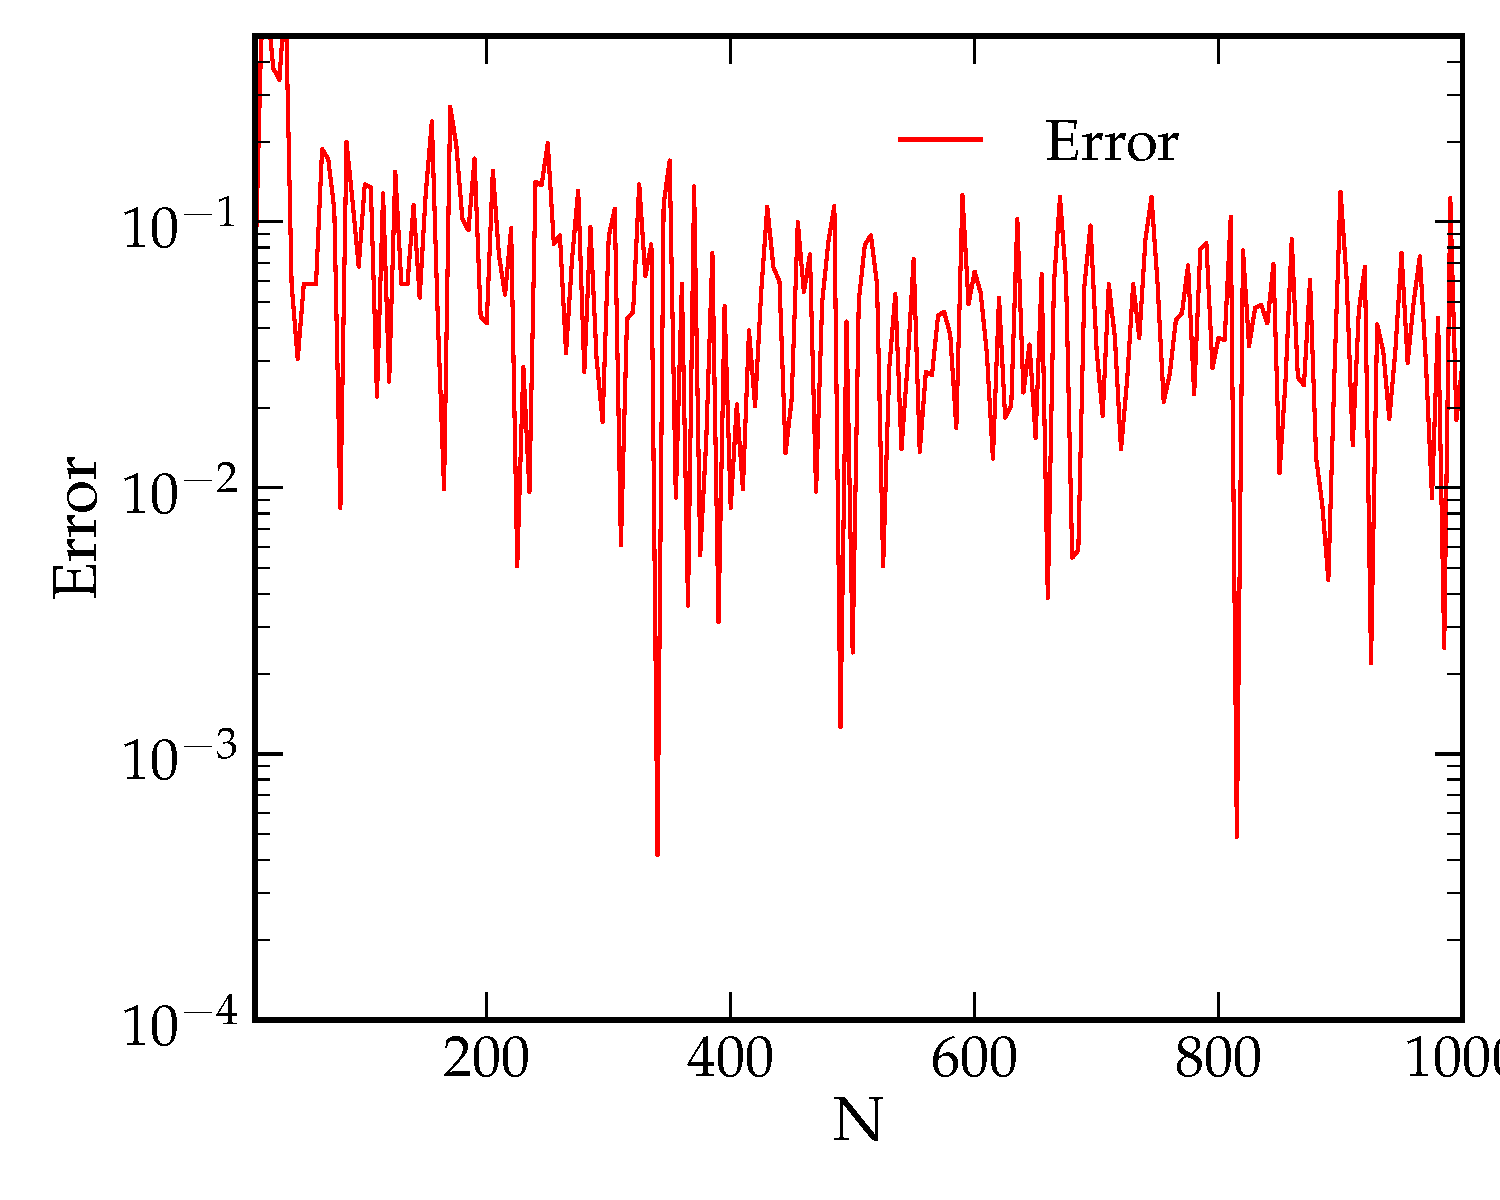
\includegraphics[width=0.5\textwidth]{1b.pdf}
\caption{Convergance of Pi by MC experimental methods using OS 
generated random numbers.}
\label{fig:sys}
\end{figure}

\subsection{The Birthday Paradox}

Running multiple simulations, in ~\ref{fig:birthday} we do 5000 trials,
 of groups of people with various size. We can estimate the probability that 
at least two of them will share a birthday. 
We find that it is when there are 23 people that there is a $50\%$ chance
that two people will share a birthday. 

\begin{figure}[bth]
\centering
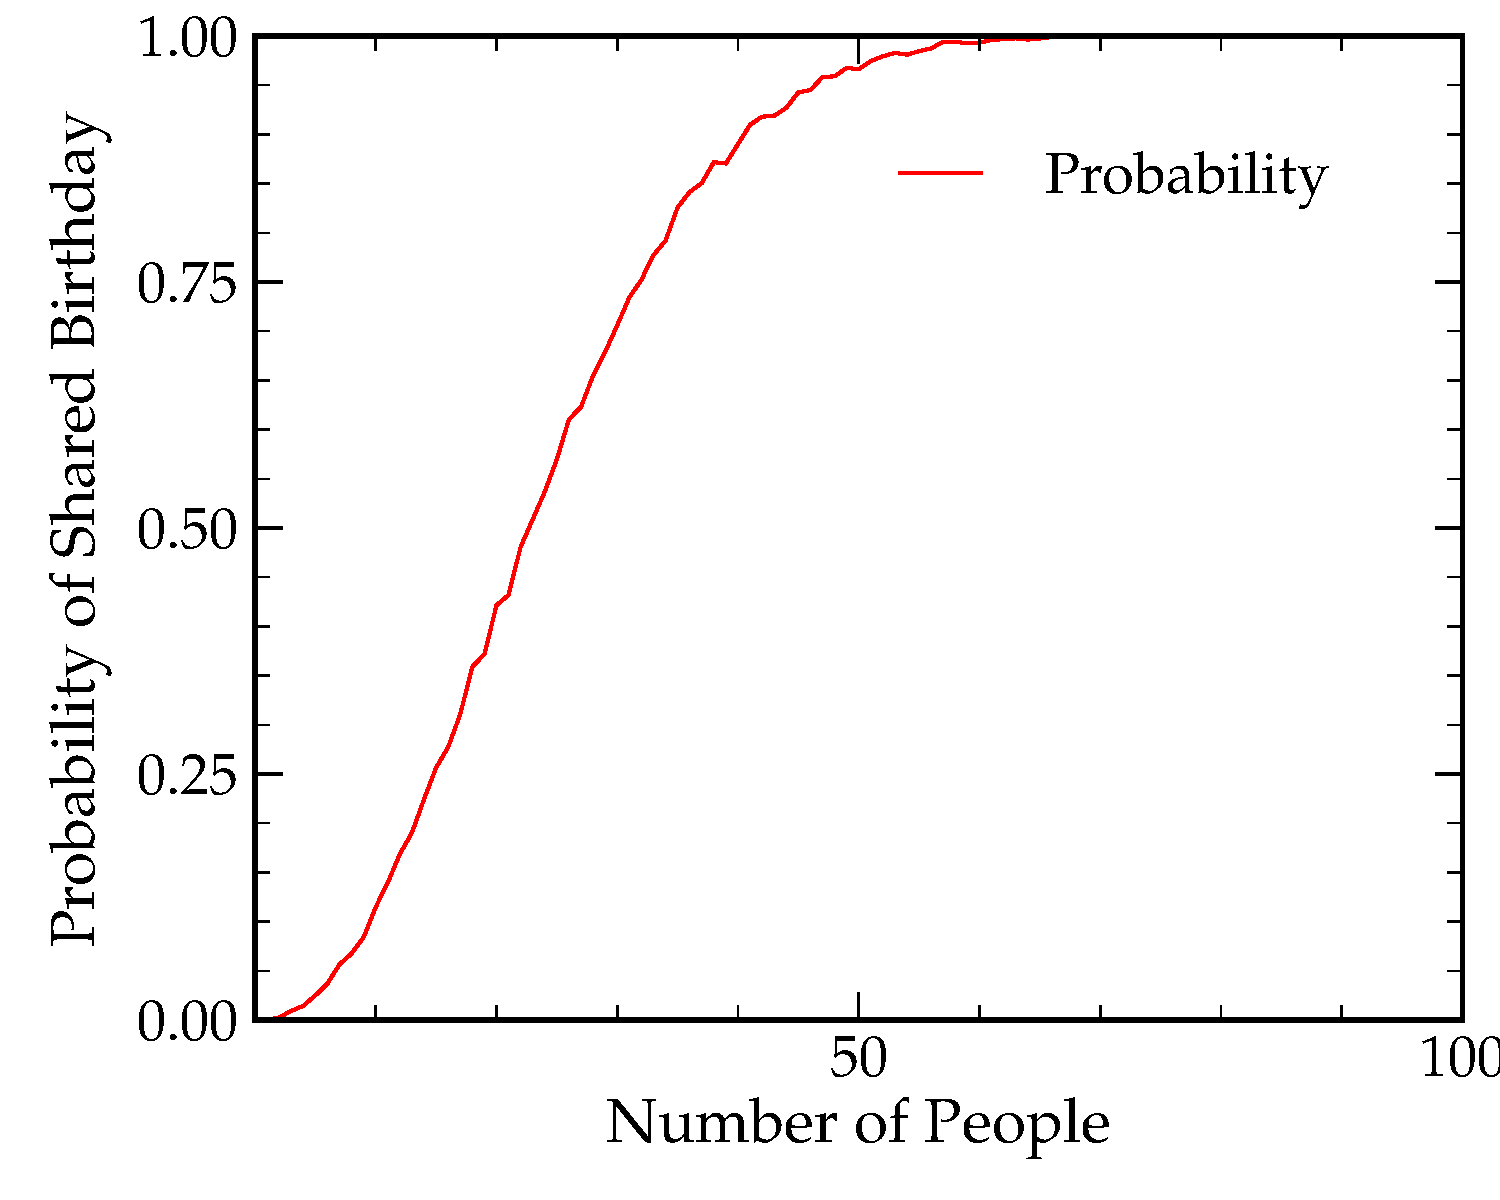
\includegraphics[width=0.5\textwidth]{2a.pdf}
\caption{The probability that at least two people out of N share a birthday. 
Assuming birthdays are uniformly distributed.}
\label{fig:birthday}
\end{figure}

\subsection{Integration}

We can use MC integration to evaluate integrals of monotonic functions over a
region. We've estimated the integral for the function $f(x) = x^2 + 1$. The
errors are shown in ~\ref{fig:integrate}. To reduce noise in the image we 
average many trials to get the average error. We can see that this method does 
converge to the correct result. However, for this simple function a method of 
direct, instead of random, estimation would be less computationally expensive.

\begin{figure}[bth]
\centering
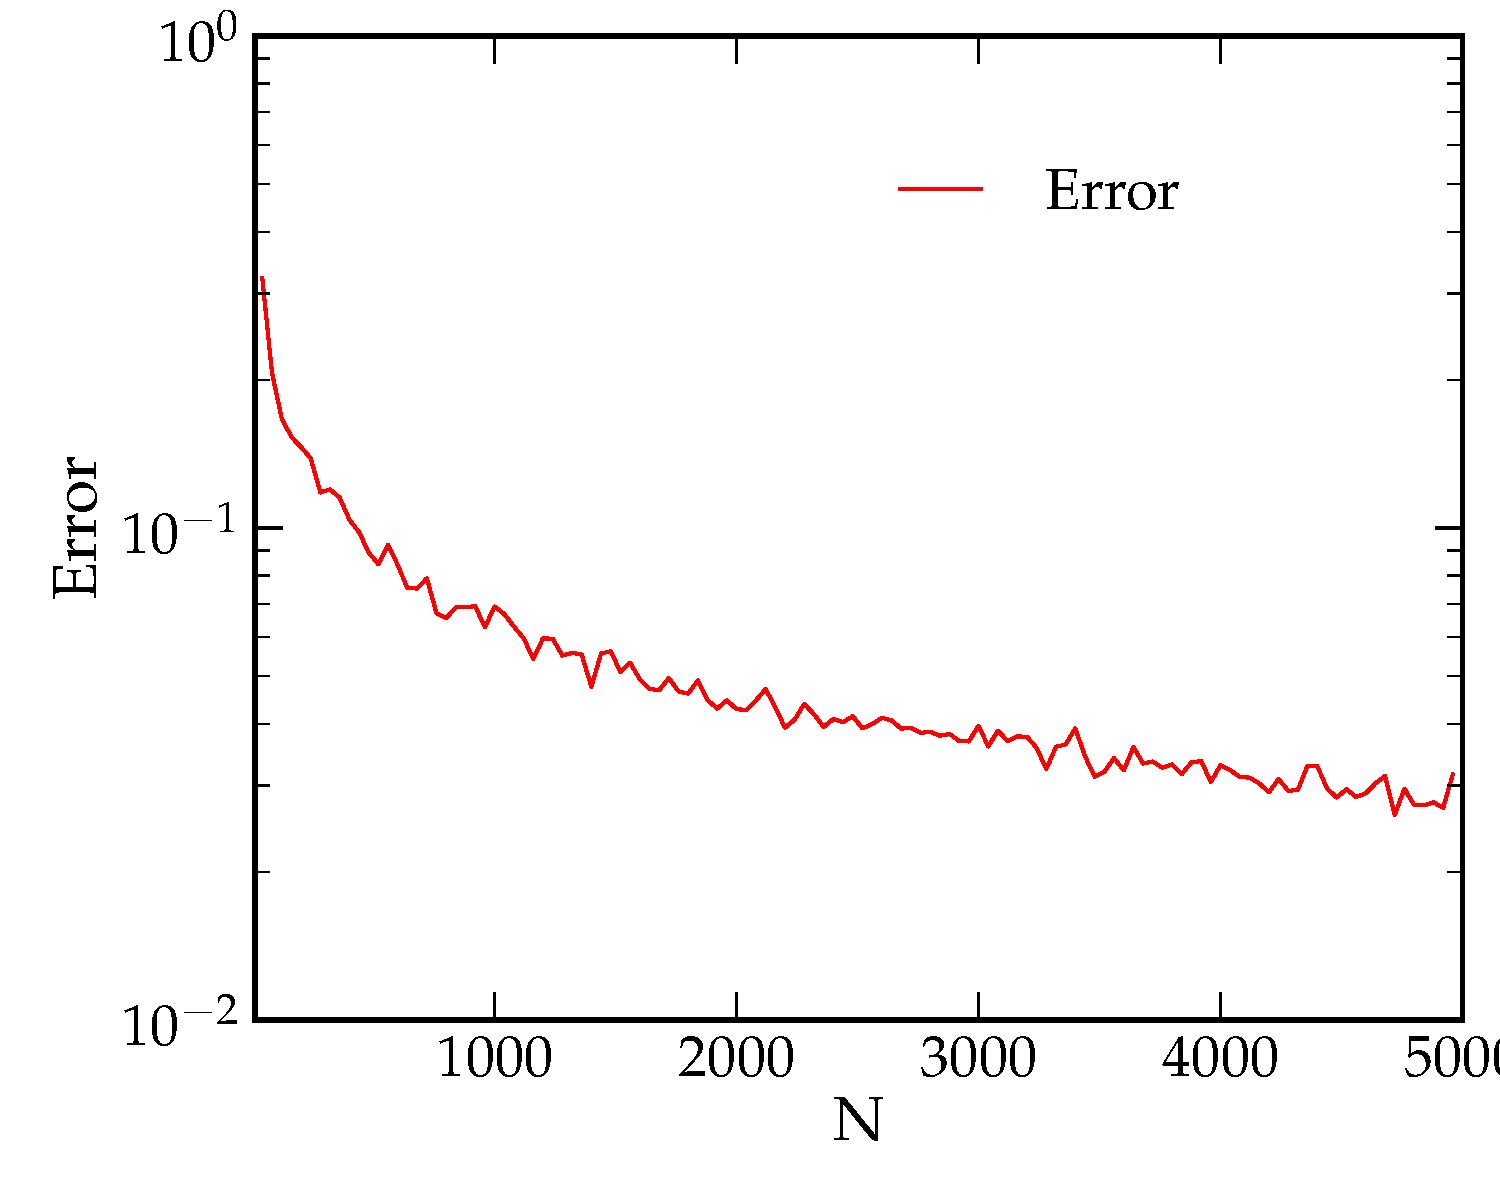
\includegraphics[width=0.5\textwidth]{3.pdf}
\caption{The average error from the true value for a given number of points.}
\label{fig:integrate}
\end{figure}


\end{document}




